\documentclass[12pt, a4paper]{article}
\title{\textbf{Laser Pointer Based Human-Computer-Interaction using Computer-Vision}}

\usepackage[labelformat=empty]{caption}
\usepackage{graphicx}
\usepackage{indentfirst}
\usepackage{wrapfig}
\usepackage{listings}
\usepackage{hyperref}
\usepackage{mathtools}
\usepackage{pgfgantt}
\usepackage{tocloft}
\usepackage{tocbibind}

\hypersetup{
	hidelinks = true
}

\begin{document}
	\listoffigures
	\pagenumbering{roman}
	\newpage
	\tableofcontents 
	\newpage
	\pagenumbering{arabic}

\section{Introduction}
\subsection{Background}
Projector systems project on the screen the contents of the computer connected to it. By the use of various technologies, we can increase the interactivity of projector systems. 

Looma is a portable projection system that uses an infra-red wand to navigate the screen. This system was built by Village Tech Solutions(VTS). Looma is being researched to make it affordable and low power consuming audio-visual technology device which will provide an interactive window to internet and access to educational contents to village schools that have never seen computers, or in some cases, even books. 

\begin{wrapfigure}{r}{0.5\textwidth}
	\centering
		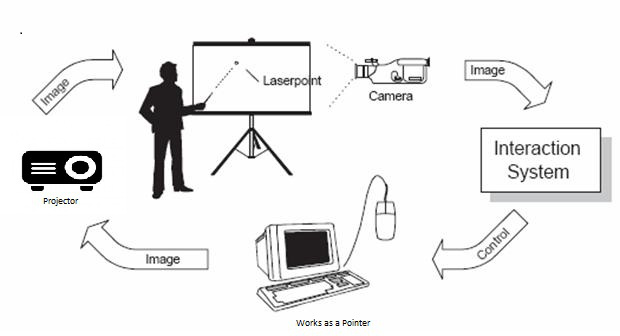
\includegraphics[width=0.48\textwidth]{abc.jpg}
	\caption{Laser Pointer based Interactive Projector System}
\end{wrapfigure}

Our project is trying to improve the interactivity and the cost of the existing Looma system such that it can be afforded by rural schools. If there is a camera used to capture the projection area, and which locates the position of the pen or other visual tools, this would be an interactive projector system. With the use of a camera, and laser pen, our project gets scoped under \textbf{Human Computer Interaction(HCI)}. \textbf{Computer Vision(CV)} is an integral part of the interaction. This vision based HCI acts as an apt mediator between the user and the computer. Here, along with images and their enhancements, the system would be emulating human vision(examples: object recognition, tracking,etc.).

\newpage
\section{Objectives:}

The basic objectives of our project is the modification of Project Looma in aspects listed below:

\begin{itemize}
	\item To make prototype for an alternative type of vision-based HCIs (Human Computer Interaction)
	\item To use laser pointer instead of IR (Infra-red) based interactive tool
	\item To remove the Wii technology, and its dependencies used in current prototype thereby, making the system efficient and cost effective
\end{itemize}


\newpage
\section{Literature Review}
The current prototype can run off a rechargeable 12V battery, has the capability to access the World Wide Web, has readily available offline content, via established partnerships, and has an extremely easy to use interface. The device is contained in a single unit with replaceable external components (i.e. keyboard, remotes), consumes less than 100 W of power, and will cost only USD 300. The system is about the size of a shoebox. 
As seen in the Figure 2, the existing Looma system functional parts can be listed as:
\subsection{Looma and Wand Details}
\begin{itemize}
\item300 lumens projector
\item Internet Connected 
\item Wireless Wand control from front of room
\item Audio output for large room setting
\item Rechargeable 12V battery (8Hrs per charge)
\item Computer: Pandaboard
\item External ports: 1 Ethernet
\item Custom power supply (12V in 5V, 12V, 19.5V out)
\item Hacked Wii IR Camera and Wii wands
\end{itemize}
\begin{figure}[htp]
\centering
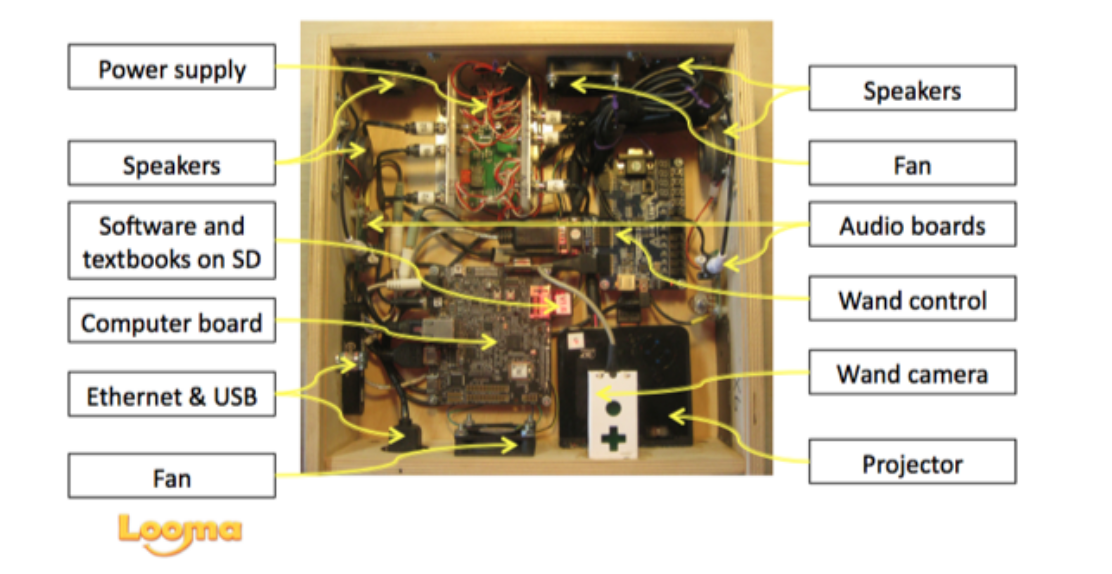
\includegraphics[scale=0.22]{looma.png}
\caption{Hardware and Electrical parts of Looma system}
\label{}
\end{figure}
\newpage
Wand control descriptions:

\begin{itemize}
\item Wand shown in the figure is a 3D printed IR light source
\item The wand design uses 555 timer to turn the IR light source on/off at a pre-determined frequency such that the blink can be interpreted as a click on the device
\item Current design uses Nintendo Wii IR camera, which are scavenged from Wii motes
\end{itemize}
\begin{figure}[htp]
\centering
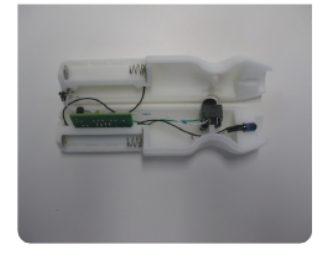
\includegraphics[scale=0.4]{wand1.png}
\caption{3D printed hacked Wii Remote wand}
\label{}
\end{figure}


\subsection{System Operation Description}
The existing system uses Wii Remote to interact in the audio-visual device. This system uses an Wii IR camera which picks up the infrared light source, and tracks it using its MOT (Multi-Object Tracking) processor present in the camera chip as shown in the Figure 4. Wii IR Camera gives out a pre-set I2C address so the interface board needs an I2C multiplexer. To convert the I2C output to serial, and to demultiplex the signals, the system has been using an FPGA board. 

\begin{figure}[htp]
\centering
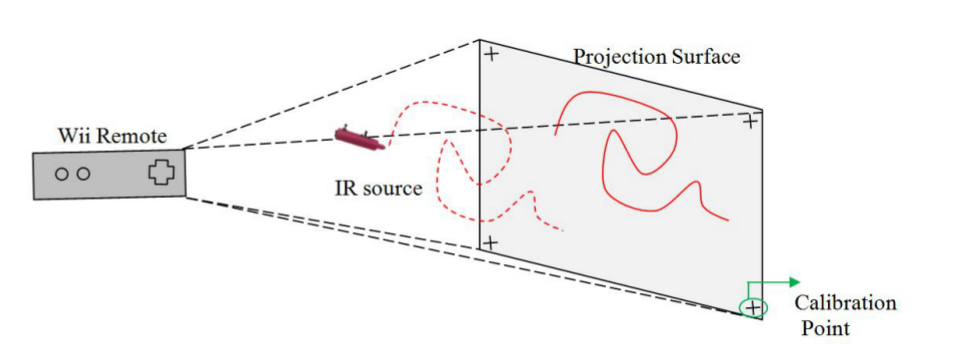
\includegraphics[scale=0.35]{wiiiii.png}
\caption{Illustration of how the movement of infrared is picked up by the Wiimote}
\label{}
\end{figure}
\subsection{Problem Statement}
 However, some of the system issues which can not be ignored are:
\begin{itemize}
\item \textbf {Drawing in the Whiteboard:} While drawing in the LOOMA software, the tracking of the IR led is very unreliable and the drawings are not made as expected.
\item \textbf{Use of Pre-built MOT processor:} There is the use of inbuilt MOT processor in the camera chip, which does part of the image processing and tracking and sending coordinates. In the case of errors, its response can not be modified to remove errors which makes it inefficient
\item \textbf{Errors not detectable:} Since the Wiimote used IR to move the mouse, the location of the IR on the screen is not visible with the naked eye thus making errors not detectable 
\item \textbf{Unavailability in the market:} Wiimote IR camera chip being used in the system can not be readily bought in the open market which makes it difficult to mass produce the system
\item \textbf{Coverage and Difficult to Interact:} Wii wand is not interactive enough and works effectively only within the projected screen space which makes interacting with the screen difficult and not intuitive

\end{itemize}

In short, hacked Wii Remotes along with the FPGA board has been adding up to the cost significantly. In addition, the system is not very stable and is inefficient to use as points aforementioned, thereby leading to the research on alternative vision-based HCIs and our project is an effort to get a prototype of one such alternative.

\newpage
\section{System Block Diagram}
\begin{figure}[htp]
\centering
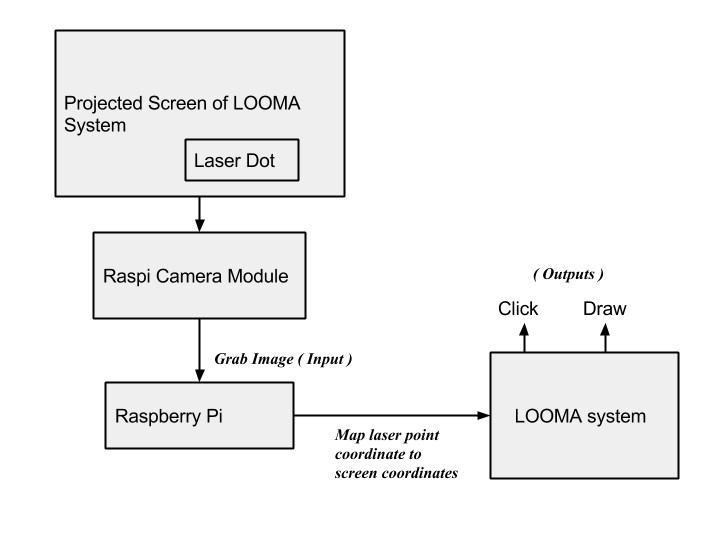
\includegraphics[scale=0.45]{block_diagram.png}
\caption{Block Diagram of the working of our system}
\label{ }
\end{figure}
\subsection{System Block Explanation}
\subsubsection{Projected Screen of Looma}

The Looma software runs on Looma hardware or Ubuntu. The display resolution of the screen is given by X = 1280 and Y = 768, and the display width is 60. Once the device is up, there are options of whether to use the wand or not use the wand. In the projected screen of Looma, ther is a custom made user interface for the teaching materials for the students as seen in Figure 6 below.

\begin{figure}[htp]
	\centering
		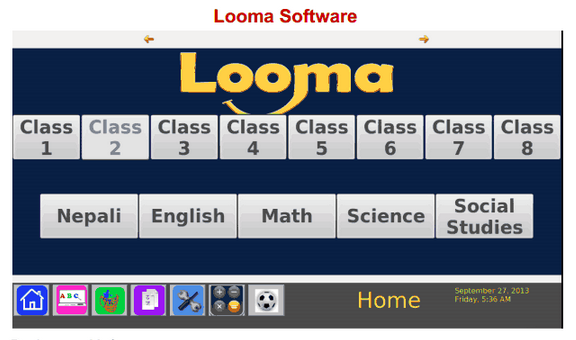
\includegraphics[scale=0.19]{loomasoftware.png}
	\caption{Looma Software}
\label{}
\end{figure}

\subsubsection{Raspi Camera Module}
Raspberry Pi Camera Board Module supports a full HD (High Definition) video streaming at fps of 30 with its 5 megapixel native resolution, and the sensor capable of 2592-1944 pixel static images. Raspberry Pi Camera Board Module was opted instead of normal USB web camera. 

The software of Raspberry Pi utilizes Rpi GPU (Graphical Processor Unit) when using Raspi Camera Module. So for example encoding \emph {h.264}, video has low impact on the CPU (Central Processor Unit) usage. Also, it has an excellent resolution of 5 Megapixels, which is higher than most USB webcams. It also has an excellent daytime image quality. If we use USB Webcam, it will have a very slow frame rate video and the CPU usage will be quite high. RPi does not have enough CPU horsepower to do higher frame rates, resolution and advanced video compression. 

\subsubsection{Using Picamera}
Raspberry Pi camera module will use \emph{Picamera 1.2} by Dave Hughes, recently released on February 06, 2014. This is a pure Python interace to the camera module. Having this interface is a boon since, up until now, the command line syntax needed to be utilized for taking still images and video taking and any changes to the camera's intrinsic features would have required a restart of the camera interfaces and Rpi.

\subsubsection{Raspberry Pi}
Raspberry Pi is a single-board computer with processor, memory, I/O ports and many more features, which together make it a functional computer for a wide range of applications in robotics. It is so simple than any logical person can program it, even it is for the first time when you work with a single-board computer.The ARM powered minicomputer is a platform with enormous possibilities and powerful enough to run many of the same programs as computer. Raspberry Pi serves as a wonderful platform for computer vision algorithms given its size, wonderful camera board and portability. Using the Picamera module, we took raw byte streams of the projected screen, and converted them to OpenCV (Open Computer Vision) object before doing further image processing algorithms.

\subsection{System Design and Description}
As seen in the Figure 5 and Figure 7, the camera will be taking in the images of Looma continually and the raspberry pi will be applying the laser detection and click action detection algorithm on the images. The image processing part will be done in the raspberry pi. Initially, the projected screen must be intially checked for any distortion and warpness. Depending on the distortion, linear and non-linear screen coordinates mapping matrix will be used. If no such distortion is present, simple linear transformation matrix will be able to map the coordinates to move the mouse pointer accordingly. However, for distortion filled projected screen, non-linear mapping transformation need to analysed and assessed. Once the mapping matrix has been understood, the raspberry pi takes in the images and works on the projected screen extracted as the region of interest. Now, all the image processing algorithms will be analysed within this ROI (Region of Interest).

\begin{figure}[htp]
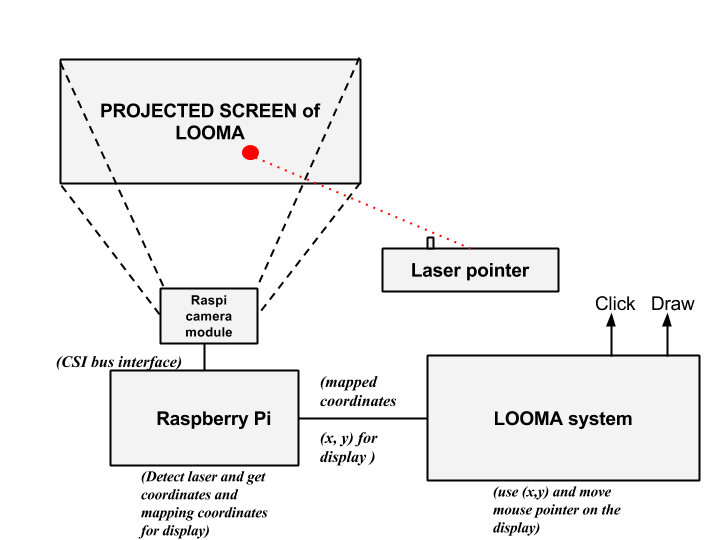
\includegraphics[scale=0.5]{proposed_system}
\caption{Proposed Block Diagram}
\label{Proposed Block Diagram}
\end{figure}

Next task is to understand the actions of the laser pointer and obtain the coordinates of it and feed it to the Looma System. The actions of the laser pointer are either simple pointing or clicking. Simple pointing will be based on the tracking of the laser pointer in the projected screen and updating the mouse pointer. Clicking of the laser pointer will be understood by the software when the laser pointer is turned on and off for a certain number of times. This on and off pattern of the laser pointer is checked in a number of frames on the same location in the image. This will be implemented as a software click and the mouse click action is done in the Looma software. 


In the Looma System, we will have the system taking in our actions and coordinates and updating its mouse pointer to do the desired mouse actions. Raspberry Pi will be connected to the Looma system through the USB to Serial Port converter wire, with the USB being the part of Raspberry Pi and the Serial Port being the part of the Looma System.

\newpage
\section{Works Accomplished in the 7th Semester}
\subsection{Detection of Laser Pointer and Mouse Movements}
	Integrating the above the codes of laser pointer detection and mouse handler into one, we were able to move the mouse pointer as per the laser pointer coordinates. Assuming that the camera captures the image from the wall without distortion, a simple linear transformation was carried out, where the laser pointer position in the image taken was mapped to the display resolution of our computer. 

	From the camera's capture properties, we have extracted the width and height of the image being captured. A simple scalex and scaley have been derived with 1366 and 766 being the display resolution of our sample display device. Once the laser pointer coordinates are found, the transformation is carried out and the mouse pointer coordinates is updated simultaneously so as the laser pointer moves, the mouse pointer coordinates gets updated and it moves with the laser motion. 
	
\begin{enumerate}
	\item \textbf{HSV segmentation:}

	In the process to detect the laser pointer we used the HSV segmentation and performed histogram analysis and obtained results as shown in Figures 11 and 12 below.
	The basic steps followed were:
	\begin{itemize}
	\item Capture the frame at each instant of time.
	\item As the captured image in opencv is in RGB (Red Green Blue) form as default , we convert it into HSV value.
	\item From the HSV value we made the value of the red color of the pointer as the default such that it can be used for further operations.
	\end{itemize}
	\emph {Why is HSV used instead of RGB value?}
	HSV separates the color component and the image intensity because of which we can operate on each image intensity as per our requirement without changing the color information which plays a vital role in color detection. RGB is the way computers treats color, and HSV try to capture the components of the way humans perceive color.   
	\item \textbf{Masking the image:}
		We obtained the threshold of the laser pointer’s color. Using the threshold range, the mask was created. The image and the masked image were operated with bitwise AND operation. Now, only the laser pointer remains in the image, remaining section is masked as black.

	\item \textbf{Canny Edge detection:}
For the edge detection we used canny edge detection algorithm.It is a multi-stage algorithm and we will go through the following stages:
\begin{enumerate}
\item \textbf {Noise Reduction}
Since edge detection is susceptible to noise in the image, first step is to remove the noise in the image with a 5x5 Gaussian filter.
\item \textbf{Finding Intensity Gradient of the Image}
Smoothened image is then filtered with a Sobel kernel in both horizontal and vertical direction to get first derivative in horizontal direction (Gx) and vertical direction (Gy). From these two images, we can find edge gradient and direction for each pixel as follows:
\begin{figure}[htp]
\centering
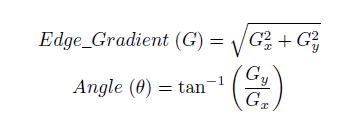
\includegraphics[scale=0.7]{canny.png}
\caption{Intensity Gradient and Direction}
\label{}
\end{figure}

Gradient direction is always perpendicular to edges. It is rounded to one of four angles   representing vertical, horizontal and two diagonal directions.
\item \textbf{Non-maximum Suppression}
After getting gradient magnitude and direction, a full scan of image is done to remove any unwanted pixels which may not constitute the edge. For this, at every pixel, pixel is checked ­if it is a local maximum in its neighborhood in the direction of gradient.

\item \textbf{Hysteresis Thresholding}
This stage decides which are all edges are really edges and which are not. For this, we need two threshold values, minVal and maxVal. Any edges with intensity gradient more than maxVal are sure to be edges and those below minVal are sure to be non-edges, so discarded. Those who lie between these two thresholds are classified edges or non-edges based on their connectivity. If they are connected to “sure-edge” pixels, they are considered to be part of edges. Otherwise, they are also discarded.
\end{enumerate}
\item \textbf{Contours:}
We found the contours of the laser, and its histogram plot was analysed as shown in the figure below.
\end{enumerate}


\begin{figure}[htp]
	\centering
	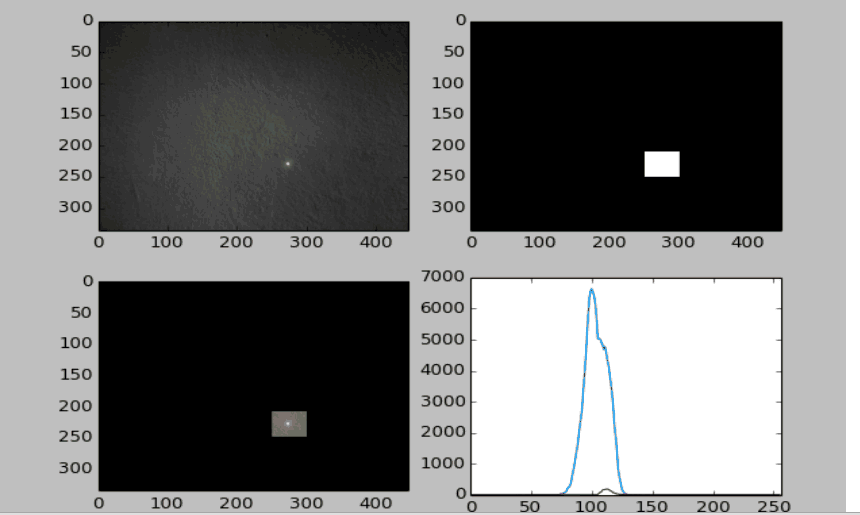
\includegraphics[scale=0.35]{histogram.png}
	\caption{Histogram Analysis of Laser Pointer}
	\label{}
\end{figure}

\subsection{Dynamic Exposure Correction}
	Correct exposure configuration of the camera can improve the color detection of laser spot. In Raspberry Pi, dynamic exposure correction was done as per need by modifying its camera capture property, which is its camera exposure compensation parameter. Here, the projected screen was captured, and the camera exposure value were modified until color of laser spot was the brighest color in the inpurt image. On every frame captured, the average of the value channel of the image was compared with the preset threshold for seeing laser spot. If the average of the value channel was greater than this threshold,the camera exposure level was decreased accordingly. A sample exposure correction code can be viewed on Appendix A4.

\subsection{Porting of Code to Raspberry Pi}
	All the codes run and tested in our computer using inbuilt webcam was ported to Raspberry Pi and run using picamera module for using the Raspberry Pi Camera Board Module. A sample picamera module code for converting to OpenCV object has been shown in Appendix A5.

\subsection{Design Calculations of 555 timer}

	A simple led circuit is used for the pointing purpose in the wand. To avoid leaving the wand on at all times, a circuit break can be introduced using a simple one-way switch. However, for the clicking purpose, the led circuit must be modified for the system to understand and implement the click. 
	One of the method to signify a click is to switch off the led for a short time but this leads to misintended clicks whenever the led is out of sight of the system. Thus, in order to avoid such errors, the led is made to blink for a specific number of times at a predetermined frequency which is understood by the system as a click. In order to implement this, a flashing led circuit was designed using a 555 timer. 
	The 555 timer is operated in astable mode and outputs rectangular pulses of certain frequency. The frequency is determined by the values of components kept in between the pins of the timer. See Fig 13 and 14.


	The values of R1, R2 and C are set to obtain the required positive time interval(T1), negative time interval(T2) and frequency(f). The calculations are made as follows:

	\noindent
	T1 (ms) = 0.693 * ( R1 + R2 ) * C \\
	T2 (ms)  = 0.693 * R2 * C \\
	Frequency (KHz)  = 1.44 /( ( R1 + R2 + R2 ) * C)

\begin{figure}[htp]
	\centering
	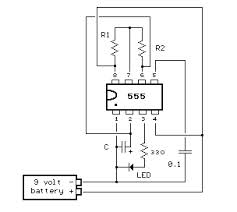
\includegraphics[scale=0.67]{blinking.jpg}
	\caption{555 Timer Calculation}
	\label{}
\end{figure}

\begin{figure}[htp]
	\centering
	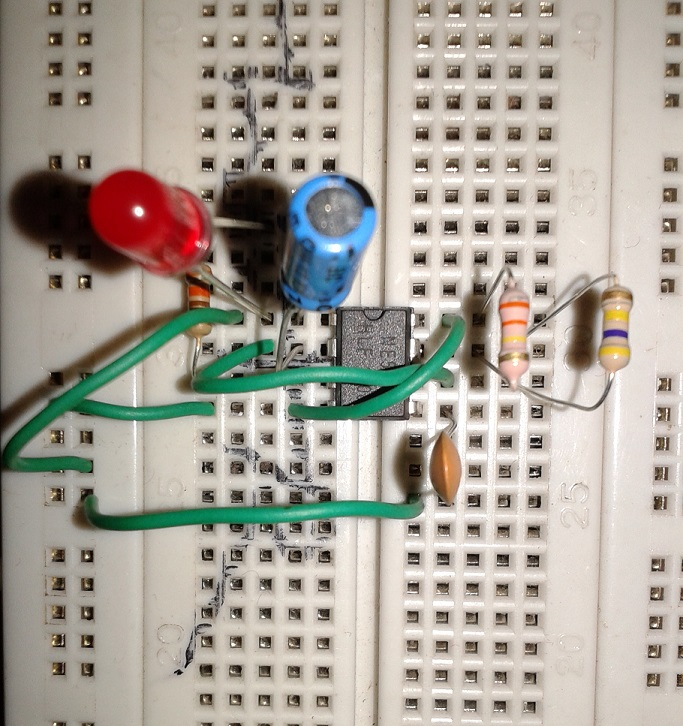
\includegraphics[scale=0.15]{circuit.jpg}
	\caption{Circuit Test on breadboard}
	\label{}
\end{figure}

	The values of the resistors and capacitor were varied until the required frequency and blinking intervals were obtained.
	By observation, we found out that R1 should be greater than 1K and C must be greater than 0.0005 uf for a proper working circuit.


\newpage

\section{Works Accomplished in the Eighth Semester}
	
\subsection{Calibration of Projected Screen}
	The image projected on the screen is not equal to the size of the computer image, but all the operations and analysis are to be performed with respect to the computer display(or camera frame). So for the calibration of the projector image, we need to map the point in the projector slide to pixel on the camera frame such that all the operations are done on the camera frame. For this mapping purpose, single projective transform is used as the matrix. Our main calibration is done on the basis of the linear mapping which works on the undistorted straight projection screen.
	However, sometimes, the projected screen in the image has some perspective distortion. Our projected screen is a quadrilateral. The actual four points of the projected screen is used as destination and perspective transform is applied which finds out the transformation matrix for corners of the quadrilateral to the destination coordinates. The following algorithm was implemented in recovering the distorted quadrilateral object.
\begin{enumerate}
\item Canny Edge Detection to obtain the edge map
\item Contours Detection to obtain the parent contour
\item Get the four corners of the parent contour
\item Get the centroid of the four corners
\item Determination of Top left, Top right, Bottom left, Bottom right points
\item Apply the perspective transformation to a destination coordinates
\end{enumerate}
	
\begin{figure}[htp]
	\centering
	
\includegraphics[scale=0.20]{looma1.png}
	\caption{Distorted Projected Screen}
	\label{}
\end{figure}

\begin{figure}[htp]
	\centering
	
\includegraphics[scale=0.20]{result.png}
	\caption{Perspective Transform Correction}
	\label{}
\end{figure}

	
\subsection{Finalization of Laser Detection Algorithm}
	In the last semester, the laser pointer had been detected using Hue-Saturation-Value(HSV) color based segmentation for red color. However, the projected screen comprises of many bright red regions which may be perceived  as white by the camera. So, the exposure correction of the camera was done dynamically based on the intensity of image taken, such that the only bright spot on the screen is the laser spot. We have applied the HSV segmentation for white color in the Value range of 200-255, and its coordinates are obtained. 
	
\subsection{Microcontroller to generate laser pulses}

	We used an avr microcontroller instead of 555 timer so that we would not need to work with resistor values and capacitors to change the frequencies and duty cycles intermittently. Microcontroller allows us to change the values on the fly and a simple burn would allow us to change the circuit behaviour in a jiffy. Below, is the schematic of our circuit. We have implemented a circuit, that keeps laser on once power is turned on, and when the push button is pressed, it sends out a pulse at a frequency set in the microcontroller. The schematic diagram of our circuit can be followed below, and the schematic as well.
	

\begin{figure}[htp]
	\centering
	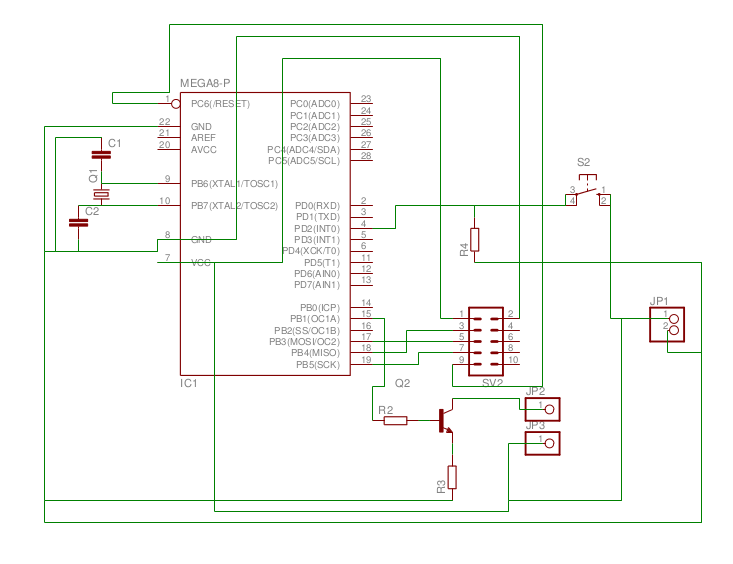
\includegraphics[scale=0.25]{schematic.png}
	\caption{Laser circuit schematic diagram}
	\label{}
\end{figure}

\begin{figure}[htp]
	\centering
	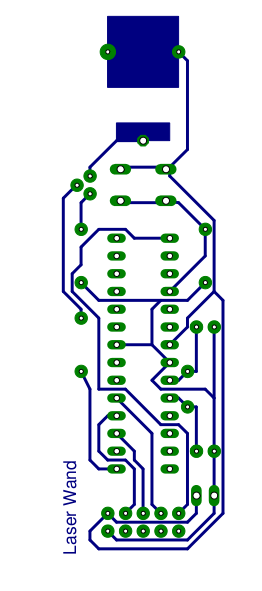
\includegraphics[scale=0.20]{eagle-non-mirror.png}
	\caption{Laser circuit eagle design diagram}
	\label{}
\end{figure}

	The laser circuit has been programmed such that it produces a 6Hz pulses when the push button is pressed, else it stays on. The target frequency has been set to 6Hz. The prescaler used is 64. The top value for pulse width modulation is obtained as, clock frequency/target frequency*scaler - 1. For a 20\% duty cycle, the on time of the laser is set to 20\% of the top value and off time is set to the 80\% of the top value. We have kept the push button switch in the interrupt pin, so that when the button is pushed, interrupt is obtained and the subsequent Interrupt Service Routine(ISR) can be run. This ISR does the work of producing PWM pulses of 20\% duty cycle. The diagram below is our working circuit.

\begin{figure}[htp]
	\centering
	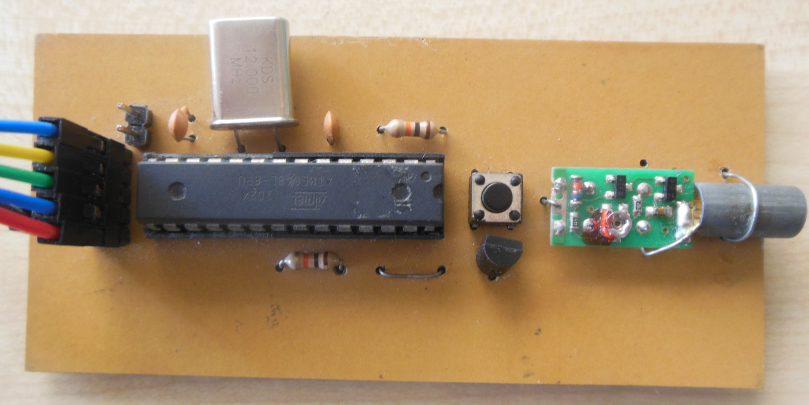
\includegraphics[scale=0.15]{front.png}
	\caption{Laser circuit front}
	\label{}
\end{figure}

\begin{figure}[htp]
	\centering
	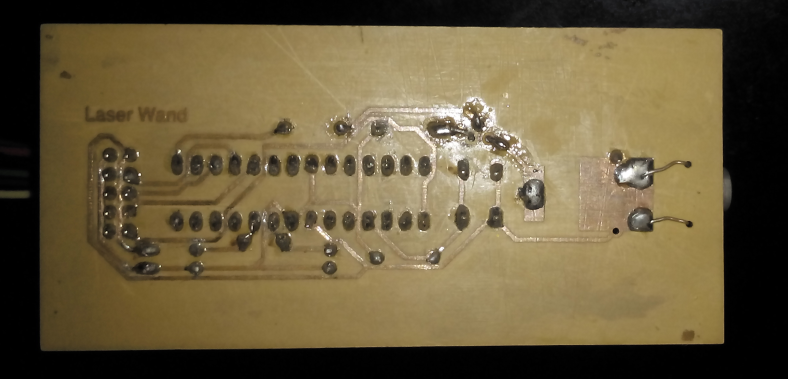
\includegraphics[scale=0.15]{back.png}
	\caption{Laser circuit back}
	\label{}
\end{figure}


\subsection{Finalized algorithm for click and drag}
	We constructed a State Diagram with the following states of laser.
\begin{enumerate}
\item Laser-off
\item Laser-on
\item Toggle-0to1
\item Toggle-1to0
\end{enumerate}

	\textbf {Laser-off} is a state of continual five or more off laser states, which occurs when the laser is not detected. \textbf{Laser-on} is a state of continual five or more on laser states, when the laser is detected. \textbf{Toggle-0to1} occurs when laser state toggles from off state to on state, whereas in \textbf{Toggle-1to0}, laser state toggles from on state to off state. 
	
	At all times, when laser is in the on state, the mouse pointer continuously moves. When laser state toggles, either from laser on to off or vice-versa, the mouse pointer is pressed. And when this mouse pointer is moving and also if the mouse pointer is in the toggled state, then the mouse starts dragging. This continues until a laser-off state or laser-on state occur, which is interpreted as a mouse release. Similarly, at every toggle state, mouse down occurs and if laser-on or laser-off state is immediately succeeded to this event, then mouse is released. This will be interpreted as click.
	
\subsection{Communication between computer and RPi}
	Currently, the Looma software is obtaining the mouse coordinates through its serial port from the FPGA board. However, we implemented a protocol for communication using Transmission Control Protocol(TCP) via ethernet to communicate the mouse actions and coordinates to the computer. The Looma board was made a server, and the Raspberry Pi board a client. The client sends the coordinates of the detected laser spot, and the actions associated with it. Accordingly, the server which is listening to the client, receives the coordinates and their respective actions. 

\subsection{Documentation}
	All the researches and case studies conducted will be documented using standard Latex documenting software.

\newpage
\section{Works Remaining in the Eighth Semester}
\subsection{Effective Algorithm implementation}
	The algorithm has been finalized and has been implemented in code but needs proper testing and evaluation in order to make it work effectively.

\begin{figure}[htp]
\centering
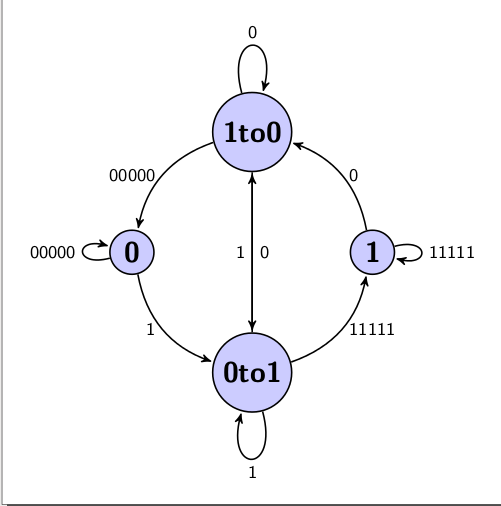
\includegraphics[scale=0.3]{state.png}
\caption{State Transition Diagram of Algorithm}
\label{}
\end{figure}

\subsection{Using the Python-Xlib library for mouse}
	The mouse coordinates as well as the actions interpreted need to be fed to the Python-Xlib for the appropriate mouse movements in the Looma board. After the client sends in the coordinates and the actions to the server present in the Looma board, the server parses the data and uses it to run the appropriate library functions.

\subsection{Documentation}
	All the remaining works and progresses will be documented using Latex, the documentation software. 

\newpage
\section{Project Timeline}
\subsection{Works Completed Timeline 7th Semester}
\begin{figure}[htp]
\centering
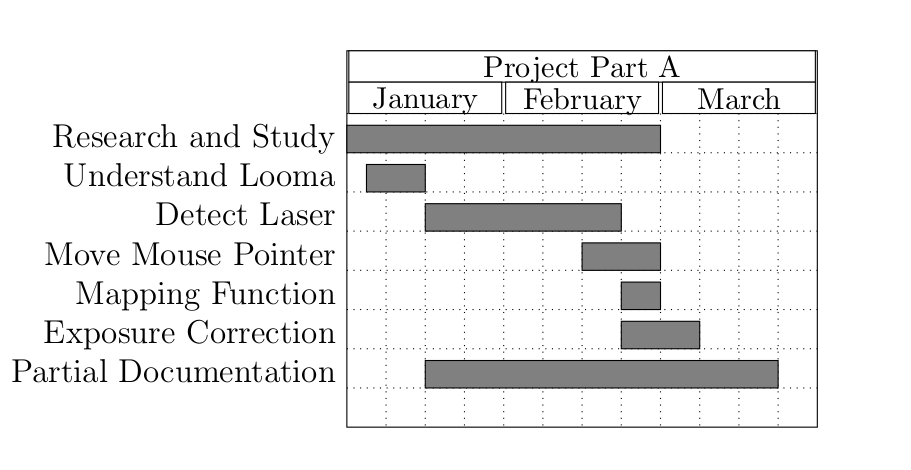
\includegraphics[scale=0.35]{reformed1.png}
\caption{Works Completed Timeline 7th Semester}
\label{}
\end{figure}
\subsection{Works Completed Timeline 8th Semester}
\begin{figure}[htp]
\centering
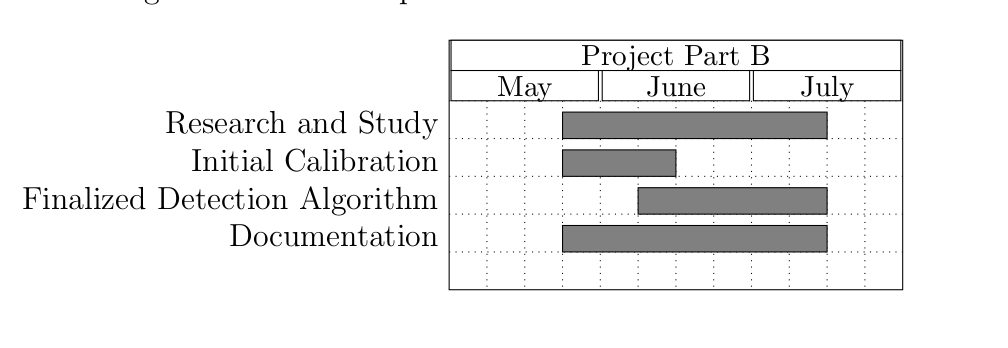
\includegraphics[scale=0.35]{come8.png}
\caption{Works Completed Timeline 8th Semester}
\label{}
\end{figure}
\newpage
\subsection{Works Remaining Timeline 8th Semester}
\begin{figure}[htp]
\centering
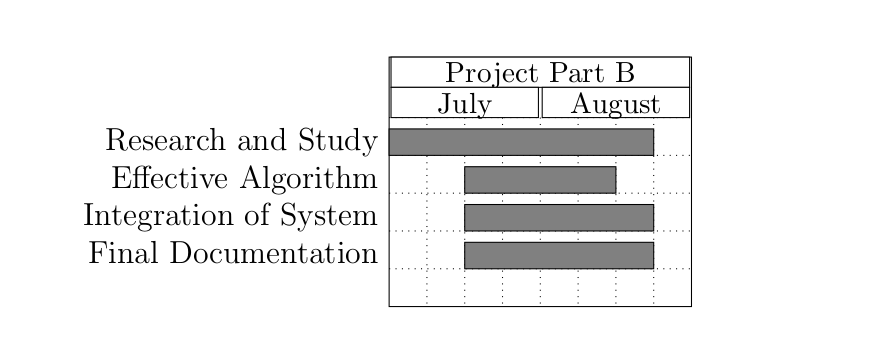
\includegraphics[scale=0.4]{remain8.png}
\caption{Works Remaining Timeline 8th Semester}
\label{}
\end{figure}

\newpage
\section{Bibliography}
\begin{enumerate}
\item Kirstein and Muller, Interaction with a Projection Screen Using a Camera-Tracked Laser Pointer,University of Dortmund, Germany
\item Mikawa, M., Morimoto, Y., Tanaka, K.: Guidance method using laser pointer and gestures for librarian robot, IEEE-RO-MAN, September, 2010
\item Johnny Chung Lee, Hacking the Nintendo Wii Remote, Carnegie Mellon University, IEEE-CS,2008 
\item Kent L. Norman, Kirk D. Norman, University of Maryland, Comparison of Relative Versus Absolute Pointing Device2, May, 2010
\item Matej MESKO, Stefan TOTH, Laser Spot Detection, University of Zilina, Faculty of Management Science and Informatics (2013) 
\end{enumerate}

\newpage
\section{References}
\begin{itemize}
	\item \url{www.python.org}
	\item \url{www.raspberrypi.org}
	\item \url{www.simplecv.org}
	\item \url{www.villagetechsolutions.org/}
	\item \url{www.docs.opencv.org/}
\end{itemize}

\end{document}
